\subsection{Entropía de acuerdo al tiempo transcurrido}

Durante la captura de los paquetes de las diferentes redes, basándose en los dos modelos definidos anteriormente, se calcularon las entropías en cada segundo transcurrido. Por lo que, de esta manera, se pudo obtener las entropías definidas por los modelos en cada momento. Esto permite observar cual sería el tiempo óptimo de escucha de la red para poder obtener un porcentaje constante de entropía. Es decir, a partir de que momento la entropía de la red no presenta grandes cambios, ya que el comportamiento de la red se vuelve casi constante, sin modificaciones importantes. 

Se presentarán, a continuación, los gráficos representativos del valor de la entropía con el paso del tiempo. Cabe destacar, que, a pesar de que se encuentren en un mismo gráfico, los valores de entropía de un modelo no puede ser comparado con el del otro, ya que ambos modelos presentar una fuente de información completamente distinto. Además, la entropía fue calculada y almacenada para cada segundo pasado, pero para mejor claridad en la presentación de los resultados, se muestran únicamente las mediciones realizadas cada 30 segundos. 

\subsubsection{Red Hogareña}
En esta red se realizaron mediciones durante 15 minutos y se puede observar el gráfico resultante:

\centerline{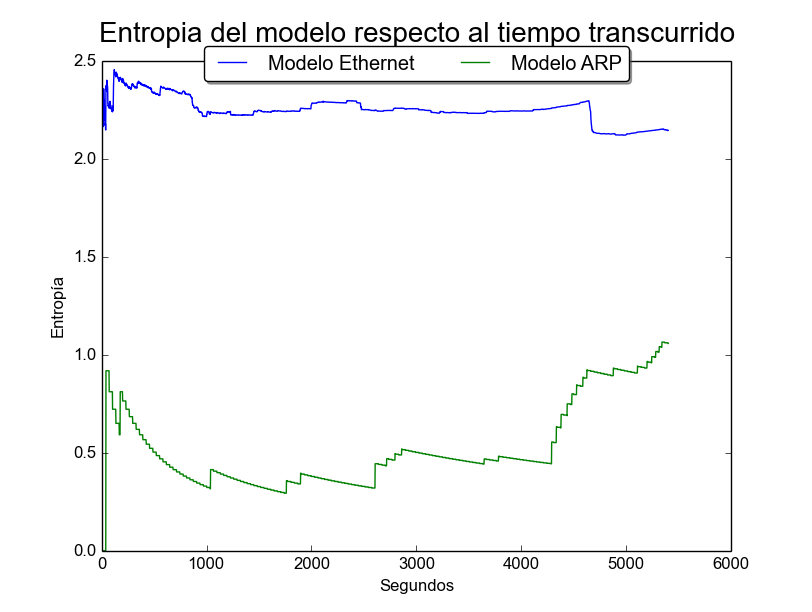
\includegraphics[width=0.8\textwidth]{./graficos/entrophyVSTime/casa_mari.png}}

En el caso del modelo Ethernet, la entropía es constante casi desde el comienzo de las capturas, ya que los paquetes enviados y recibidos aumentan de manera proporcional para todos los símbolos. De esta manera la cantidad de "ruido" existente en la red no es modificada. En el caso del Modelo ARP para esta red específica, se puede denotar que aún no se realizaron las capturas el tiempo suficiente como para encontrar la entropía constante del mismo. 

\subsubsection{Red Laboratorio}
Esta red fue capturada durante quince minutos, debido a la cantidad de datos acumulado para ese tiempo fue importante. 

\centerline{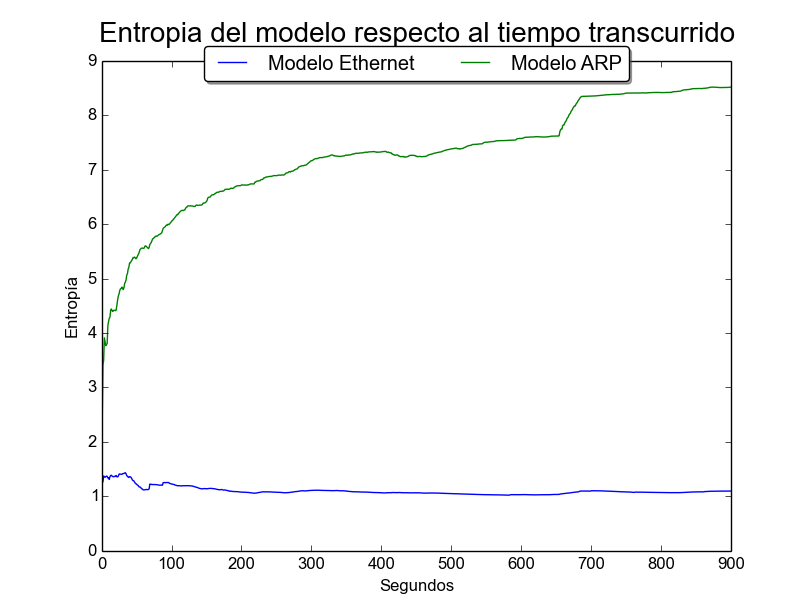
\includegraphics[width=0.8\textwidth]{./graficos/entrophyVSTime/labo5.png}}

Se puede notar que la entropía del Modelo Ethernet actua de manera constante casi desde un comienzo, similar al caso de la Red Hogareña. En el caso de los valores de información para el Modelo ARP, aún no se puede definir el valor constante del mismo. 

\subsubsection{Red Devartis}
Luego de realizar capturas durante una hora se puede observar el siguiente resultado. 

\centerline{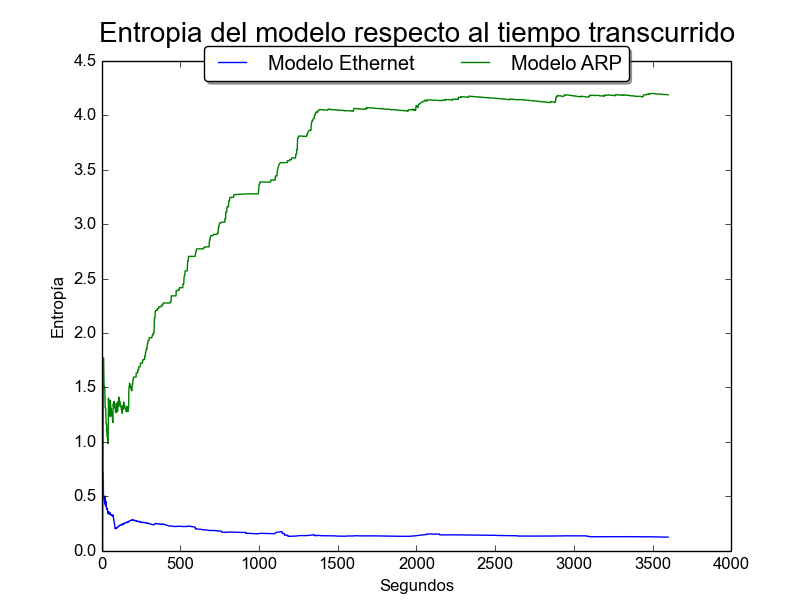
\includegraphics[width=0.8\textwidth]{./graficos/entrophyVSTime/laburo_mari.png}}

Este caso actúa de manera similar a los casos anteriores para el Modelo Ethernet. En el caso de la entropía resultante para el Modelo ARP se observa claramente la constación del mismo a partir de los 25 minutos. Luego de transcurrido ese tiempo, la misma aumenta pero paulatinamente. 


\subsubsection{Red Mercap}
Al igual que la red anterior, se realizan capturas de los paquetes de la red durante una hora. 

\centerline{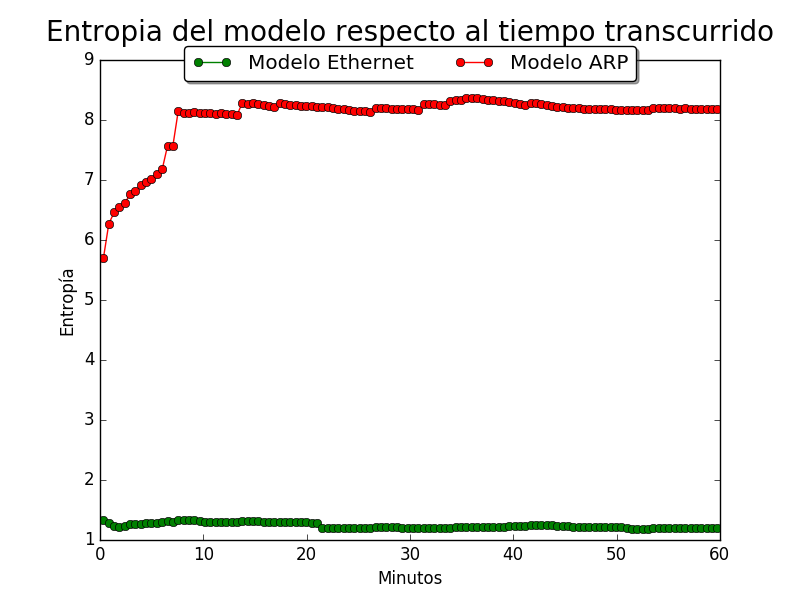
\includegraphics[width=0.8\textwidth]{./graficos/entrophyVSTime/laburo_eze.png}}

Bastaba, tanto para la entropía del Modelo Ethernet como el de ARP con realizar mediciones durante 10 minutos, ya que luego no se presentan importantes modificaciones en el medio. 

Cabe destacar el comportamiento constante de la entropía del Modelo ARP que siempre presenta un valor mayor al del otro modelo. Para justificarlo, hablaremos de los símbolos presentados para cada fuente de información. El Modelo Ethernet consiste en el evento "un paquete de un determinado type", y, por lo observado en las capturas (Ver sección \ref{"Type"}), la cantidad de símbolos es baja. La máxima cantidad de símbolos observados, dentro de una red, es de 4, por lo que al aplicarse el cálculo de la entropía, el valor resultante será bajo. Por el otro lado, el Modelo ARP, por lo analizado en la sección \ref{"Grafos"}, presenta un importante y notorio número de símbolos diferentes, generando así un valor alto de entropía. 